%Die Angabe des schlauen Spruchs auf diesem Wege funtioniert nur,
%wenn keine Änderung des Kapitels mittels den in preambel/chapterheads.tex
%vorgeschlagenen Möglichkeiten durchgeführt wurde.
\chapter{Evaluation of results}
\label{chap:chapter6}
%\vspace{-3cm}
%\vspace{2cm}
This chapter presents results of classification using the experimental setup described in chapter~\ref{chap:chapter6}. The term \emph{classification accuracy} of a class used in this chapter is defined as,

\[ \begin{array}{ll} \mbox{classification accuracy}(l_i) = \frac{\mbox{Samples correctly predicted as $l_i$}}
								{\mbox{Total samples with label $l_i$}}
							\times 100 & 
							\forall \,l_i \in \{\mbox{\texttt{P,I,T}}\} 
	\end{array}\]

Where, $l$ is the label of test sample $x=\{\boldsymbol{x},l\}$.

In the presented evaluation, the cross-validation accuracy defined in the section~\ref{sec:impl:tr} is also noted for each set of the experiments, as this is the value of accuracy during the self-validation of much larger training set.

All experiments performed are done after selecting optimal values of $C$ and $\gamma$, obtained using grid search. In the first part of this chapter, the classification accuracy for each of the kernel in \texttt{LIBSVM} is evaluated, to check their performance for different fault types and in presence of transient noise. The second part tries to explore the possibility of optimizing the classifier for yield or quality of product. This is done with help of experiments carried out by improving accuracy levels of one type of faults at the expense of the others. The third part explores two possibilities - that of using one of the using a single prediction model for predicting all types of circuits, and the second, to use a model trained with a known circuit to classify test data from new, unknown circuits.

\section{Classification of permanent faults}
\label{sec:wp}
When a test pattern is able to detect permanent fault in the circuit, running the same pattern again would result in same faulty output every time. Hence it is easy to detect a permanent fault in the circuit. This is also shown to be true in the literature survey presented in the chapter~\ref{chap:chapter2}. Hence, in the experimental evaluation the sample population and test data are pre-screened for permanent faults before the classifier is trained.

Consider a the case, where the value of fault reproducibility defined in the section~\ref{sec:secfs}), $\epsilon = Test Runs$. In our classification problem this can mean,
\begin{enumerate}
  \item It is a permanent fault.
  \item A rare case of highly repetitive intermittent fault, and can be assumed to be \enquote{critical}.
  \item An extremely rare case of a transient fault, as it happened at the same location and for same input test pattern, in all of the test runs.
\end{enumerate}

In the other direction, for permanent faults the value of $\epsilon = Test Runs$ holds true, except a rare possibility that the transient noise affects all of the test patterns, which have resulted in a failure at POs, in at least one of the test runs. This is also an extremely rare possibility. Hence we assume that, a fault is permanent if and only if $\epsilon = Test Runs$.

If we go back to the section~\ref{sec:secfs} and observe the plot for $\epsilon$ in figure~\ref{fig:epsilonp45k}, we can observe our assumption to be fairly accurate. Hence if we do a slight modification in our experimental setup and already remove faults where $\epsilon = Test Runs$, and classify them as permanent faults, we can achieve up to 100\% permanent fault classification, and we would be left with a binary classification problem between transient and intermittent faults.

There are two possibilities to do such pre-screening of permanent faults, one is just to scan all instances for all $\epsilon = Test Runs$ and remove those, or use an ensemble of two SVMs, first one to separate permanents and the other one to classify intermittents and transients. In this evaluation, first option is considered and permanents are removed from sample population, wherever analysis is done without considering permanent faults.

\section{Classification with different kernels}
The first set of experiments consist of evaluation of accuracy levels without assigning class-weights \emph{i.e.} class-weights described in section~\ref{sec:impl:tr} are assumed to be \{1,1,1\} for permanent, intermittent and transient faults respectively. The experiments are repeated for each type of kernel provided by \texttt{LIBSVM}.

This set of experiments consist of two rounds each for each kernel, first round considers permanents in the sample population. This is done to show there are indeed kernels which can classify permanent faults with an accuracy up to 100\%, in case permanents are to be discarded using an ensemble of 2 different SVM kernels. The second round evaluates classification accuracies, by discarding permanents based on $\epsilon$ from the sample population.

\subsection{Linear Kernel}
The accuracy of SVM using a linear kernel is summarized in table~\ref{tab:linwp} with considering permanent faults in the sample population, and the same considering permanents are discarded based on $\epsilon$, is summarized in the table~\ref{tab:linwop}.
\begin{table}[h]

	\captionsetup{justification=centering}
\begin{tabular}{ccccccc}
\hline
\multicolumn{1}{c}{\multirow{3}{*}{Circuit}} & \multicolumn{6}{c}{Accuracy (\%)}\\ \cline{2-7} 
\multicolumn{1}{c}{}                         & \multicolumn{1}{c}{\multirow{2}{*}{Cross-validation}} & \multicolumn{2}{c}{Permanent} & \multicolumn{2}{c}{Intermittent} & \multicolumn{1}{c}{\multirow{2}{*}{Transient}} \\ \cline{3-6}
                                             &                                                       & w/o noise     & with noise    & w/o noise      & with noise      &                                                \\ \hline
p45k                                         & 90.14                                                 & 87.50         & 87.50         & 77.50          & 64.58           & 93.90                                          \\
p100k                                        & 87.38                                                 & 100           & 100           & 80.95          & 57.14           & 95.91                                          \\
p141k                                        & 83.89                                                 & 98.21         & 98.21         & 61.90          & 57.14           & 100                                            \\
p267k                                        & 85.12                                                 & 100           & 100           & 55.00          & 52.50           & 100                                            \\
p279k                                        & 89.52                                                 & 98.30         & 96.61         & 78.94          & 52.50           & 89.79                                          \\
p295k                                        & 89.84                                                 & 100           & 100           & 81.39          & 65.11           & 100   \\
\hline                                        
\end{tabular}
\caption {Classification accuracy for linear kernel}
\label{tab:linwp}
\end{table}

In both cases, with and without permanent faults, it can be observed that permanent faults are being relatively accurately classified and the background transient noise seem to have almost no effect on the classification accuracy of permanent faults. Intermittent faults in both cases have relatively low accuracy levels and tend to deteriorate severely in presence of transient noise. 


\begin{table}[h]
\captionsetup{justification=centering}
\begin{tabular}{ccccc}
\hline
\multirow{3}{*}{Circuit} & \multicolumn{4}{c}{Accuracy (\%)}\\ \cline{2-5} 
                         & \multirow{2}{*}{Cross-validation} & \multicolumn{2}{c}{Intermittent} & \multirow{2}{*}{Transient} \\ \cline{3-4}
                         &                                   & w/o noise      & with noise      &                            \\ \hline
p45k                     & 87.81                             & 72.91          & 70.08           & 97.95                      \\
p100k                    & 81.43                             & 69.05          & 59.52           & 97.96                      \\
p141k                    & 84.13                             & 78.57          & 76.19           & 100                        \\
p267k                    & 77.09                             & 80.00          & 55.00           & 100                        \\
p279k                    & 84.65                             & 78.94          & 52.63           & 91.83                      \\
p295k                    & 89.17                             & 90.69          & 81.39           & 100           \\
\hline            
\end{tabular}
\caption {Classification accuracy for linear kernel, without permanent faults}
\label{tab:linwop}
\end{table}

After removing permanents from the sample population, classification accuracies are observed to improve, with an exception of p100k. However, accuracy levels are observed to increase for intermittents with noise, even in the case of p100k. The classification accuracy of transient faults has also increased. Cross-validation accuracy levels have decreased, as a large chunk of correctly classified data in the earlier case was permanent faults. Comparatively lower accuracy levels for intermittent faults and almost 100\% classification rate for transients suggests that the linear kernel is more biased towards transient faults.

\subsection{Polynomial Kernel}
\begin{table}[h]

	\captionsetup{justification=centering}
\begin{tabular}{ccccccc}
\hline
\multirow{3}{*}{Circuit} & \multicolumn{6}{c}{Accuracy (\%)}\\ \cline{2-7} 
                         & \multirow{2}{*}{Cross-validation} & \multicolumn{2}{c}{Permanent} & \multicolumn{2}{c}{Intermittent} & \multirow{2}{*}{Transient} \\ \cline{3-6}
                         &                                   & w/o noise     & with noise    & w/o noise      & with noise      &                            \\ \hline
p45k                     & 90.92                             & 87.50         & 89.58         & 68.75          & 70.83           & 83.67                      \\
p100k                    & 89.70                             & 100           & 97.82         & 69.04          & 66.66           & 93.87                      \\
p141k                    & 87.94                             & 100           & 100           & 73.80          & 71.42           & 95.00                      \\
p267k                    & 87.34                             & 100           & 96.55         & 82.50          & 60.00           & 85.71                      \\
p279k                    & 91.42                             & 98.30         & 96.55         & 81.57          & 73.68           & 91.83                      \\
p295k                    & 90.78                             & 100           & 98.21         & 76.09          & 72.09           & 95.91      \\
\hline                                                     
\end{tabular}
\caption {Classification accuracy for polynomial kernel}
\label{tab:polywp}
\end{table}

The accuracy of SVM using a polynomial kernel is summarized in table~\ref{tab:polywp} with considering permanent faults in the sample population, and the same considering permanents are discarded based on $\epsilon$, is summarized in table~\ref{tab:polywop}.

The accuracy of classification of permanent faults, without noise in case of the polynomial kernel is observed to be even higher than that for linear kernel. For permanents with noise, classification rates are almost similar. Intermittent faults and permanents without noise in first round, are deteriorating in some cases, while improving significantly in others. With noise, however, accuracy of intermittent fault classification is improved. Classification accuracy of transient faults has decreased as compared to the linear kernel.

\begin{table}[h]
\captionsetup{justification=centering}
\begin{tabular}{ccccc}
\hline
\multirow{3}{*}{Circuit} & \multicolumn{4}{c}{Accuracy (\%)}\\ \cline{2-5} 
                         & \multirow{2}{*}{Cross-validation} & \multicolumn{2}{c}{Intermittent} & \multirow{2}{*}{Transient} \\ \cline{3-4}
                         &                                   & w/o noise      & with noise      &                            \\ \hline
p45k                     & 87.81                             & 81.25          & 72.91           & 87.76                      \\
p100k                    & 85.00                             & 78.57          & 66.66           & 89.79                      \\
p141k                    & 85.57                             & 80.95          & 76.19           & 100                        \\
p267k                    & 81.38                             & 82.50          & 72.50           & 93.87                      \\
p279k                    & 85.57                             & 78.94          & 73.68           & 93.87                      \\
p295k                    & 92.28                             & 93.02          & 86.04           & 93.87                      \\
\hline
\end{tabular}
\caption {Classification accuracy for polynomial kernel, without permanent faults}
\label{tab:polywop}
\end{table}

In the second round, after removing permanents, a huge improvement in the accuracy of intermittent faults is observed as compared to the first round. The results are also better than those for the linear kernel.  A marginal improvement in the transient fault classification accuracy is also observed as compared to the first round. However, overall figures for transients are lower than those for the linear kernel. These observations suggest that, the polynomial kernel is slightly biased towards intermittents.


\subsection{RBF Kernel}

The accuracy of SVM using a Radial Basis Function (RBF) kernel is summarized in table~\ref{tab:rbfwp} with considering permanent faults in the sample population, and the same considering permanents are discarded based on $\epsilon$, is summarized in table~\ref{tab:rbfwop}.

\begin{table}[h]
\captionsetup{justification=centering}
\begin{tabular}{ccccccc}
\hline
\multirow{3}{*}{Circuit} & \multicolumn{6}{c}{Accuracy (\%)}\\ \cline{2-7} 
                         & \multirow{2}{*}{Cross-validation} & \multicolumn{2}{c}{Permanent} & \multicolumn{2}{c}{Intermittent} & \multirow{2}{*}{Transient} \\ \cline{3-6}
                         &                                   & w/o noise     & with noise    & w/o noise      & with noise      &                            \\ \hline
p45k                     & 91.21                             & 100           & 100           & 66.66          & 64.58           & 91.83                      \\
p100k                    & 87.36                             & 100           & 100           & 64.28          & 61.94           & 93.87                      \\
p141k                    & 88.63                             & 100           & 100           & 73.80          & 71.42           & 93.87                      \\
p267k                    & 87.27                             & 100           & 98.27         & 80.00          & 72.50           & 93.87                      \\
p279k                    & 89.52                             & 98.30         & 96.55         & 78.92          & 71.05           & 93.87                      \\
p295k                    & 91.00                             & 100           & 100           & 79.06          & 74.41           & 95.91                     \\
\hline                                                     
\end{tabular}
\caption {Classification accuracy for RBF kernel}
\label{tab:rbfwp}
\end{table}
The classification rates for permanent faults, with and without noise, are higher for RBF kernel as compared to others. This means that RBF can be used to screen permanent faults in pre-screening in an ensemble classifier with 2 kernels. Like in other cases, injection of the transient noise has affected the accuracy of intermittent fault classification significantly. Accuracy figures for both, intermittent faults with and without noise, are lower as compared to previous two kernels. The transient fault classification accuracy shows a marginal improvement over the polynomial kernel, but it is still lower than the linear kernel.

Intermittent fault classification accuracy is higher for smaller circuits, but shows no change for more complex ones. However, for intermittent faults injected with noise, the accuracy is improved as compared to the first round, but is still lower than other kernel types. A slight increase in transient fault classification accuracy is also observed. 

A notable observation in case of the RBF kernel is its comparatively higher cross-validation accuracy figures and lower overall classification accuracy when using test data, an indication that the kernel may be overfitting.

\begin{table}[h]
	\captionsetup{justification=centering}
\begin{tabular}{ccccc}
\hline
\multirow{3}{*}{Circuit} & \multicolumn{4}{c}{Accuracy (\%)}                                                                 \\ \cline{2-5} 
                         & \multirow{2}{*}{Cross-validation} & \multicolumn{2}{c}{Intermittent} & \multirow{2}{*}{Transient} \\ \cline{3-4}
                         &                                   & w/o noise      & with noise      &                            \\ \hline
p45k                     & 87.56                             & 77.08          & 70.83           & 91.83                      \\
p100k                    & 83.33                             & 78.57          & 64.28           & 89.79                      \\
p141k                    & 86.53                             & 83.33          & 80.95           & 100                        \\
p267k                    & 80.19                             & 82.50          & 70.00           & 92.34                      \\
p279k                    & 85.64                             & 78.92          & 76.31           & 95.91                      \\
p295k                    & 85.64                             & 79.06          & 76.31           & 95.91  						  \\
\hline
\end{tabular}
\caption {Classification accuracy for RBF kernel, without permanent faults}
\label{tab:rbfwop}
\end{table}

\subsection{Sigmoid Kernel}

The accuracy of SVM using a sigmoid kernel is summarized in the table~\ref{tab:sigwp} with considering permanent faults in the sample population, and the same considering permanents are discarded based on $\epsilon$, is summarized in the table~\ref{tab:sigwop}.

Again, the permanent fault classification rates are is fairly high, which makes the sigmoid kernel another possible candidate for an ensemble classifier using 2 SVM kernels. The intermittent fault classification accuracy is comparatively low (except p100k) despite a high cross validation accuracy. This coupled with the high transient fault classification accuracy indicate that, sigmoid kernel is biased towards transient faults. This has also resulted in a degradation of accuracy levels when intermittents were injected with transient noise.

\begin{table}[h]

	\captionsetup{justification=centering}
\begin{tabular}{ccccccc}
\hline
\multirow{3}{*}{Circuit} & \multicolumn{6}{c}{Accuracy (\%)}\\ \cline{2-7} 
                         & \multirow{2}{*}{Cross-validation} & \multicolumn{2}{c}{Permanent} & \multicolumn{2}{c}{Intermittent} & \multirow{2}{*}{Transient} \\ \cline{3-6}
                         &                                   & w/o noise     & with noise    & w/o noise      & with noise      &                            \\ \hline
p45k                     & 89.55                             & 97.50         & 97.50         & 77.08          & 60.41           & 95.91                      \\
p100k                    & 85.08                             & 100           & 100           & 95.23          & 52.38           & 71.42                      \\
p141k                    & 84.17                             & 100           & 100           & 57.14          & 57.14           & 100                        \\
p267k                    & 82.46                             & 100           & 98.27         & 42.50          & 42.50           & 100                        \\
p279k                    & 89.29                             & 98.30         & 96.55         & 81.57          & 52.63           & 87.76                      \\
p295k                    & 85.09                             & 98.21         & 98.21         & 69.76          & 65.11           & 100                       \\
\hline                                                     
\end{tabular}
\caption {Classification accuracy for sigmoid kernel}
\label{tab:sigwp}
\end{table}

The kernel became more biased towards transients when permanent fault examples were removed from the sample population. The transient fault classification accuracy was observed to increase to near 100\%. Also, the intermittent classification accuracy also increased at the same time, with and without the transient noise.

\begin{table}[h]
\captionsetup{justification=centering}
\begin{tabular}{ccccc}
\hline
\multirow{3}{*}{Circuit} & \multicolumn{4}{c}{Accuracy (\%)}                                                                 \\ \cline{2-5} 
                         & \multirow{2}{*}{Cross-validation} & \multicolumn{2}{c}{Intermittent} & \multirow{2}{*}{Transient} \\ \cline{3-4}
                         &                                   & w/o noise      & with noise      &                            \\ \hline
p45k                     & 84.46                             & 68.75          & 60.41           & 100                        \\
p100k                    & 80.00                             & 81.39          & 52.38           & 100                        \\
p141k                    & 80.04                             & 78.57          & 73.80           & 100                        \\
p267k                    & 75.17                             & 75.00          & 55.00           & 100                        \\
p279k                    & 83.41                             & 81.57          & 52.63           & 91.83                      \\
p295k                    & 92.28                             & 93.02          & 86.04           & 91.83                     \\
\hline
\end{tabular}
\caption {Classification accuracy for sigmoid kernel, without permanent faults}
\label{tab:sigwop}
\end{table}

This set of experiments show that the relative accuracy levels for the fault classification actually increase if the sample population and the test data is pre-screened for permanents faults. Hence for rest of the evaluation,  all experiments are done by considering that the sample population consists of intermittent and transient faults only.

\subsection{Analysis of intermittent fault classification}
\label{sec:wp:intanalysis}
The first set of experiments reveal that the classification accuracy for intermittent faults comparatively low as compared to the other fault types. Hence, more detailed analysis is done, which can provide some hints about the improvement of intermittent fault classification accuracy. First, an analysis is done about how fault activation rates might be affecting classification accuracy. Table~\ref{tab:intdetail} summarizes the result of this analysis and it notes the accuracy results for different intermittent fault activation rates in the test dataset. For this analysis, a subset of circuits were analyzed using all four kernels of \texttt{LIBSVM}.

\begin{table}[h]
\captionsetup{justification=centering}
\resizebox{\textwidth}{!}{%
\begin{tabular}{cccccccc}
\hline
\multirow{3}{*}{Circuit} & \multirow{3}{*}{Kernel} & \multicolumn{6}{c}{Classification accuracy (\%)}\\ \cline{3-8} 
                         &                         & \multicolumn{3}{c}{Intermittent faults without noise} & \multicolumn{3}{c}{Intermittent faults with noise} \\ \cline{3-8} 
                         &                         & rate = 0.1    & rate = 0.01    & rate = 0.001   & rate = 0.1   & rate = 0.01   & rate = 0.001  \\ \hline
\multirow{4}{*}{p141k}   & linear                  & 100           & 81.25          & 25.00          & 100          & 75.00         & 25.00         \\
                         & polynomial              & 100           & 81.25          & 37.5           & 100          & 75.00         & 25.00         \\
                         & RBF                     & 100           & 81.25          & 50.00          & 100          & 81.25         & 37.5          \\
                         & sigmoid                 & 100           & 81.25          & 25.00          & 100          & 68.75         & 25.00         \\
\hline
\multirow{4}{*}{p267k}   & linear                  & 94.73         & 82.35          & 20.00          & 89.47        & 35.29         & 0.00          \\
                         & polynomial              & 94.73         & 88.23          & 20.00          & 94.73        & 64.70         & 20.00         \\
                         & RBF                     & 94.73         & 88.2           & 20.00          & 94.73        & 58.82         & 20.00         \\
                         & sigmoid                 & 94.73         & 70.58          & 20.00          & 89.47        & 35.29         & 0.00          \\

\hline
\multirow{4}{*}{p295k}   & linear                  & 100           & 88.23          & 77.77          & 100          & 88.23         & 33.33         \\
                         & polynomial              & 100           & 94.11          & 77.77          & 100          & 100           & 33.33         \\
                         & RBF                     & 100           & 94.117         & 77.77          & 100          & 100           & 33.33         \\
                         & sigmoid                 & 100           & 88.23          & 77.77          & 100          & 76.47         & 22.22     	\\
\hline   
\end{tabular}
}
\caption{Accuracy of intermittent fault classification for different fault rates}
\label{tab:intdetail}
\end{table}

The analysis shows that accuracy levels are fairly high for high fault activation rates of intermittent faults, but go on deteriorating for lower values of fault activation rates. The main reason behind this behavior is that, at lower fault activation rates of $10^{-3}$, the behavior of transient faults (activation rates for which are $10^{-2}$ to $10^{-4}$) matches the behavior of intermittents, and the learning algorithm fails to separate them from each other. This suggests that, instances where intermittent failures occurred only once and did not repeat themselves, are not able to convey enough information in their extracted features. Hence no classification algorithm will be able to improve on these figures significantly. To further elaborate this, an accuracy analysis for the same circuits from table~\ref{tab:intdetail} is done by removing those intermittent faults from the test set, whose reproducibility ($\epsilon$) is less than one. The results of this analysis are presented in table~\ref{tab:intsweep}.

\begin{table}[h]
\begin{tabular}{ccccc}
\hline
\multirow{3}{*}{Circuit} & \multirow{3}{*}{Kernel} & \multicolumn{3}{c}{Classification accuracy (\%)}              \\ \cline{3-5} 
                         &                         & \multicolumn{2}{c}{Intermittent} & \multirow{2}{*}{Transient} \\ \cline{3-4}
                         &                         & w/o noise      & with noise      &                            \\ \hline
\multirow{4}{*}{p141k}   & linear                  & 100            & 100             & 100                        \\
                         & polynomial              & 100            & 100             & 100                        \\
                         & RBF                     & 100            & 100             & 100                        \\
                         & sigmoid                 & 100            & 100             & 100                        \\
\hline
\multirow{4}{*}{p267k}   & linear                  & 100            & 100             & 100                        \\
                         & polynomial              & 100            & 100             & 93.87                      \\
                         & RBF                     & 100            & 100             & 95.91                      \\
                         & sigmoid                 & 100            & 100             & 100                        \\
\hline
\multirow{4}{*}{p295k}   & linear                  & 100            & 100             & 100                        \\
                         & polynomial              & 100            & 100             & 93.87                      \\
                         & RBF                     & 100            & 100             & 91.83                      \\
                         & sigmoid                 & 100            & 100             & 91.83                     \\
\hline
\end{tabular}
\caption{Improvement in accuracy levels after removing intermittents with $\epsilon = 1$}
\label{tab:intsweep}
\end{table}

The analysis from table~\ref{tab:intsweep} shows that, if we remove intermittents with low fault activation rates from the test set, the classification of intermittent faults is accurate up to 100\%. The accuracy of transient fault classification remains the same, as the same classifier model and the same test dataset for transient faults is used as earlier experiments.

\section{Optimization for yield and quality using class weights}
\label{sec:ww}

Class-weights are used while training the SVM by adding a penalty to samples of particular class, to compensate for the unavailability of sufficient positive examples for that class. \texttt{LIBSVM} provides a functionality to adjust individual class weights, to bias classification towards a specified class using \texttt{-wi} switch. We can use this functionality to:
\begin{itemize}
  \item Fine-tune $C$ values for optimal classification. This way we can have a classifier which can separate most of examples in dataset.
  \item Optimize the classifier to classify one type of faults more accurately than the other.
\end{itemize}

The first point presents another possibility to improve yield and retaining quality, at the same time. This is done by balancing the training dataset. An unbalanced dataset is a possibility in our case, as we have set a tolerance of $\pm$ 75 on training examples of each class, as explained in the section~\ref{sec:gsp:configuration}. 

Table~\ref{tab:optp267k} shows the accuracy values when optimizations mentioned above are performed.

\begin{table}[h]
\captionsetup{justification=centering}
\begin{tabular}{cccccc}
\hline
\multirow{3}{*}{Kernel}     & \multirow{3}{*}{Optimization Criterion} & \multirow{3}{*}{Class-weights \{\texttt{I,T}\}} & \multicolumn{3}{c}{Classification accuracy (\%)}              \\ \cline{4-6} 
                            &                                         &                                                   & \multicolumn{2}{c}{Intermittent} & \multirow{2}{*}{Transient} \\ \cline{4-5}
                            &                                         &                                                   & w/o noise      & with noise      &                            \\ \hline
\multirow{3}{*}{linear}     & Intermittent                            & \{1.5,1\}                                         & 100            & 100             & 22.44                      \\
                            & Transient                               & \{1,1\}                                           & 80.00          & 55.00           & 100                        \\

                            & All                               & \{1.9,1.8\}                                           & 72.5          & 67.5           & 95.91                        \\
\hline
\multirow{3}{*}{polynomial} & Intermittent                            & \{1.85,1.05\}                                     & 97.50          & 80.00           & 20.00                      \\
                            & Transient                               & \{1.3,1.95\}                                      & 82.50          & 67.50           & 97.95                      \\

                            & All                               & \{1.9,1.25\}                                           & 95.00          & 78.00           & 77.5                        \\
\hline
\multirow{3}{*}{RBF}        & Intermittent                            & \{1.75,1.15\}                                     & 95.00          & 72.50           & 89.79                      \\
                            & Transient                               & \{1.2,1.3\}                                       & 72.50          & 70.00           & 95.91                      \\

                            & All                               & \{1,1\}                                           & 82.50          & 70.00           & 92.34                        \\
\hline
\multirow{3}{*}{sigmoid}    & Intermittent                            & \{1.7,1.1\}                                       & 85.00          & 77.50           & 65.30                      \\
                            & Transient                               & \{1.9,1.8\}                                       & 82.5           & 57.5            & 100                       \\

                            & All                               & \{1.7,1.75\}                                           & 82.50          & 47.00           & 100                        \\
\hline
\end{tabular}
\caption{Accuracy after class-weight optimization for p267k}
\label{tab:optp267k}
\end{table}

To find out the set of optimal values of weights in the case of optimization for both intermittent and transient faults at the same time, an exhaustive search of combinations of class-weights for \texttt{I} and \texttt{T} classes is performed. For experimental purpose, a limited search of region [1,2] with steps of 0.05 for combinations of class-weights is performed. Heat-maps for this search are shown in figure~\ref{fig:heatmap} for p267k. Using these heat-maps the weight combinations were set up for the analysis presented above.

Optimization for \enquote{All} labels is done by considering weights corresponding to the highest cross-validation accuracy. After class-weight optimization, accuracy levels are observed to be improved as compared to the same analysis done in the section~\ref{sec:wp}.


\begin{figure}
        \centering
			\captionsetup{justification=centering}
        \begin{subfigure}[h]{0.45\linewidth}
                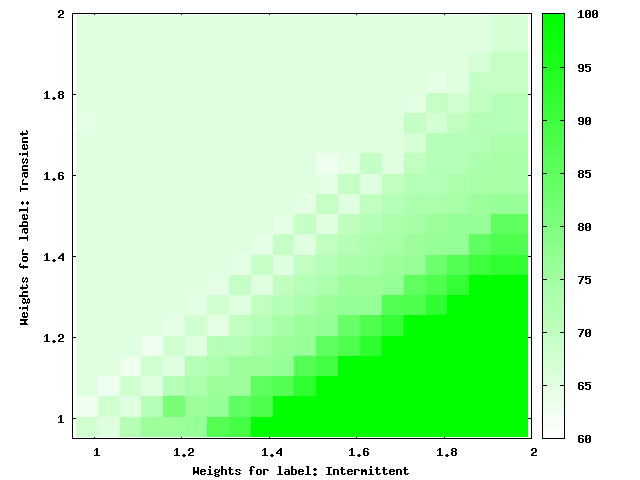
\includegraphics[scale=0.25]{figures/lin256i.png}
                \caption{Intermittent fault accuracy, linear kernel}
        \end{subfigure}
        \begin{subfigure}[h]{0.45\linewidth}
                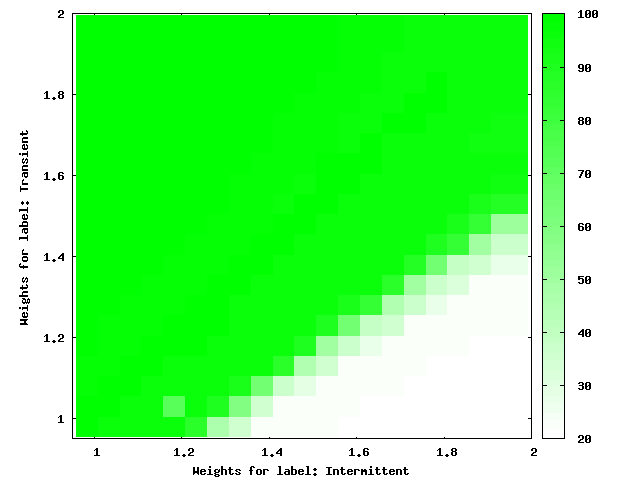
\includegraphics[scale=0.25]{figures/lin256t.png}
                \caption{Transient fault accuracy, linear kernel}
        \end{subfigure}

			\begin{subfigure}[h]{0.45\linewidth}
                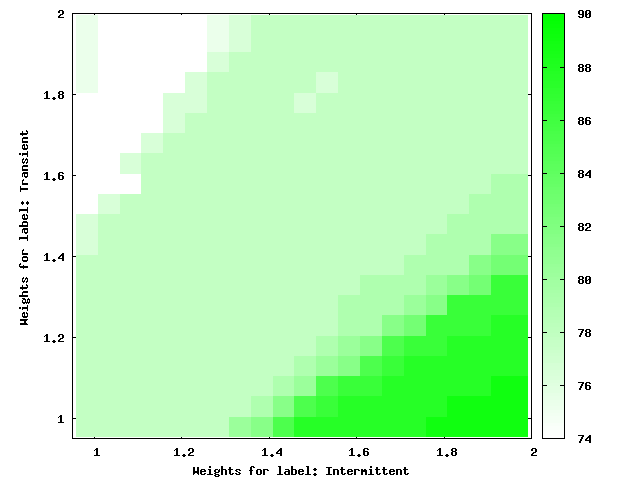
\includegraphics[scale=0.25]{figures/poly256i.png}
                \caption{Intermittent fault accuracy, polynomial kernel}
        \end{subfigure}
        \begin{subfigure}[h]{0.45\linewidth}
                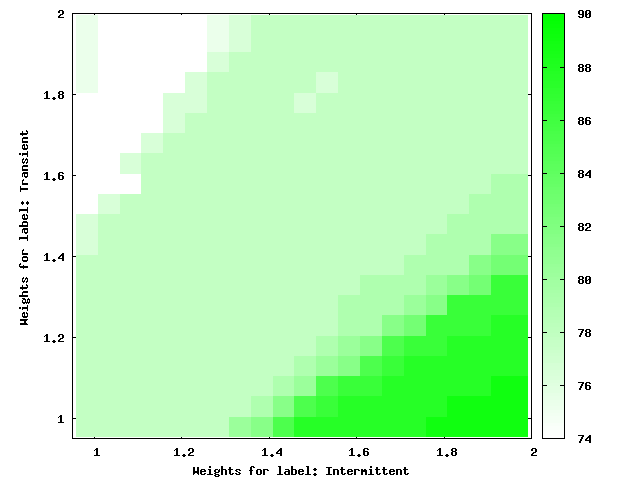
\includegraphics[scale=0.25]{figures/poly256i.png}
                \caption{Transient fault accuracy, polynomial kernel}
        \end{subfigure}

        \begin{subfigure}[h]{0.45\linewidth}
                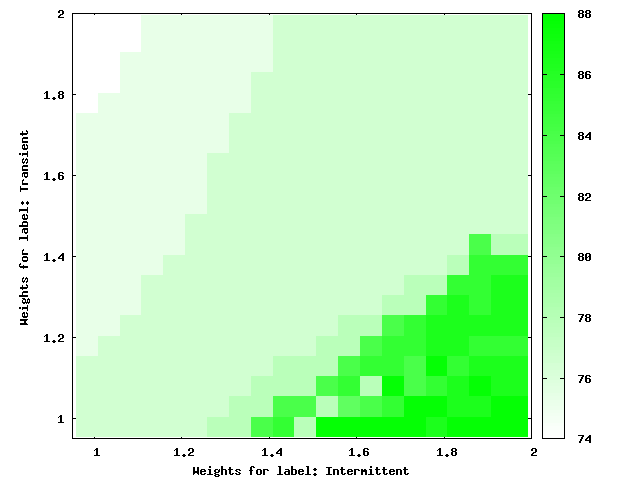
\includegraphics[scale=0.25]{figures/rbf256i.png}
                \caption{Intermittent fault accuracy, RBF kernel}
        \end{subfigure}
			\begin{subfigure}[h]{0.45\linewidth}
                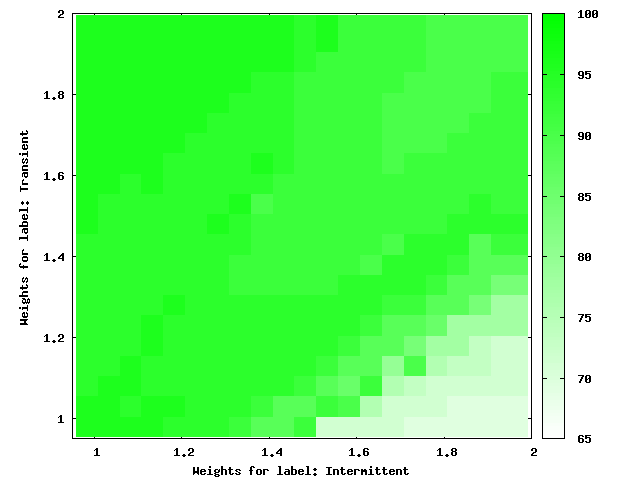
\includegraphics[scale=0.25]{figures/rbf256t.png}
                \caption{Transient fault accuracy, RBF kernel}
        \end{subfigure}

        \begin{subfigure}[h]{0.45\linewidth}
                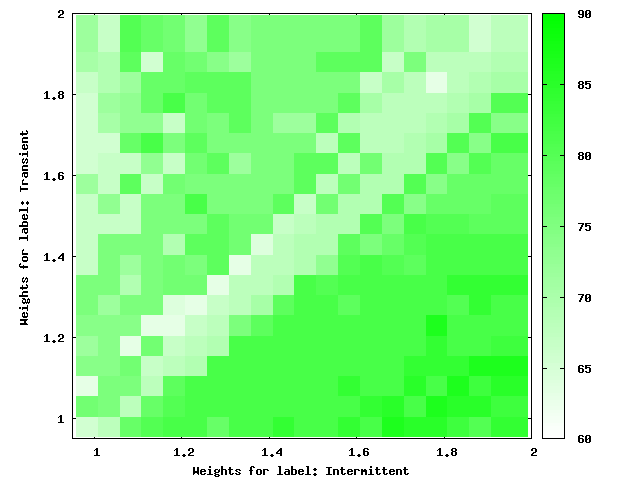
\includegraphics[scale=0.25]{figures/sig256i.png}
                \caption{Intermittent fault accuracy, sigmoid kernel}
        \end{subfigure}
			\begin{subfigure}[h]{0.45\linewidth}
                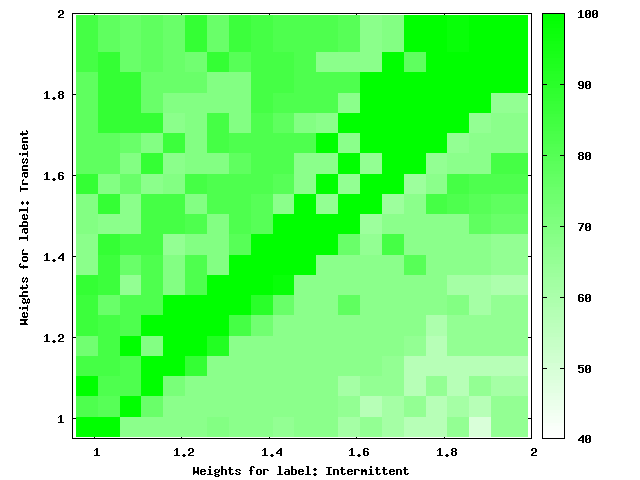
\includegraphics[scale=0.25]{figures/sig256t.png}
                \caption{Transient fault accuracy, sigmoid kernel}
        \end{subfigure}

        \caption{Plots of accuracy by varying class-weights for p256k}
        \label{fig:heatmap} 
\end{figure}



\section{Classification using extrapolation of known training datasets}
So far the evaluation of test data is done using a sample population of the same circuit. In this section two other possibilities are considered. First, to use a sample population of a known circuit, to classify the data of an another unknown circuit. Second, to have a single training dataset of all circuits, and use a classifier model built from this to predict example data of a circuit type, whose sample population is already present in this \emph{universal} dataset.

\subsection{Using single known model for classification}
In practical situations, one might not have the necessary training data for a new product beforehand, especially at the start of production. This section explores possibility of using known datasets for unknown circuit types. This set of experiments are done using the training data of p295k to predict test sets of other circuits. p295k is chosen as sample population as it provided with the relatively most accurate results in the first set of experiments. The results obtained are summarized in the table~\ref{tab:univ295k}.

\begin{table}[h]
\captionsetup{justification=centering}
\resizebox{\textwidth}{!}{%
\begin{tabular}{cccccc}
\hline
\multirow{3}{*}{Kernel}     & \multirow{3}{*}{Cross-validation accuracy (\%)} & \multirow{3}{*}{Circuit} & \multicolumn{3}{c}{Accuracy (\%)}                             \\ \cline{4-6} 
                            &                                                 &                          & \multicolumn{2}{c}{Intermittent} & \multirow{2}{*}{Transient} \\ \cline{4-5}
                            &                                                 &                          & without noise    & with noise    &                            \\ \hline
\multirow{5}{*}{Linear}     & \multirow{5}{*}{89.17}                          & p45k                     & 77.08            & 72.91         & 95.91                      \\
                            &                                                 & p100k                    & 71.42            & 64.28         & 75.51                      \\
                            &                                                 & p141k                    & 78.57            & 73.08         & 100                        \\
                            &                                                 & p267k                    & 77.5             & 62.5          & 100                        \\
                            &                                                 & p279k                    & 78.94            & 57.89         & 97.95                      \\
\hline
\multirow{5}{*}{Polynomial} & \multirow{5}{*}{90.78}                          & p45k                     & 79.16            & 81.63         & 75.51                      \\
                            &                                                 & p100k                    & 78.57            & 76.19         & 73.46                      \\
                            &                                                 & p141k                    & 88.09            & 80.95         & 91.83                      \\
                            &                                                 & p267k                    & 82.5             & 77.5          & 87.75                      \\
                            &                                                 & p279k                    & 78.94            & 76.31         & 97.95                      \\
\hline
\multirow{5}{*}{RBF}        & \multirow{5}{*}{92.28}                          & p45k                     & 79.16            & 81.25         & 73.46                      \\
                            &                                                 & p100k                    & 78.57            & 73.8          & 71.42                      \\
                            &                                                 & p141k                    & 88.09            & 80.95         & 97.95                      \\
                            &                                                 & p267k                    & 82.5             & 72.5          & 89.79                      \\
                            &                                                 & p279k                    & 78.94            & 71.05         & 100                        \\
\hline
\multirow{5}{*}{Sigmoid}    & \multirow{5}{*}{85.64}                          & p45k                     & 79.16            & 81.25         & 73.46                      \\
                            &                                                 & p100k                    & 78.57            & 73.8          & 71.42                      \\
                            &                                                 & p141k                    & 88.09            & 80.95         & 97.95                      \\
                            &                                                 & p267k                    & 82.5             & 72.5          & 89.79                      \\
                            &                                                 & p279k                    & 78.94            & 71.79         & 100                       \\
\hline
\end{tabular}
}
\caption{Accuracy by extrapolating training dataset of p295k to test other circuits}
\label{tab:univ295k}
\end{table}

The comparison of the results with those obtained in the section~\ref{sec:wp}, shows an increase in accuracy levels. This can be attributed to two factors, a comparatively more balanced dataset of p295k and high cross-validation accuracy levels of this dataset. Hence it is observed that, using a good-quality known dataset, examples from other circuit types can be classified with acceptable accuracy levels.

\subsection{Using a universal training set for classification}

In this set of experiments, a single universal sample population is built using sample populations of individual circuits. The aim of this experiment to check a possibility of building an incremental universal dataset, which is able to classify data from any of known circuit types. Table~\ref{tab:universal} summarizes results observed.

\begin{table}[h]
\captionsetup{justification=centering}
\resizebox{\textwidth}{!}{%
\begin{tabular}{cccccc}
\hline
\multirow{3}{*}{Kernel}     & \multirow{3}{*}{Cross-validation accuracy (\%)} & \multirow{3}{*}{Circuit} & \multicolumn{3}{c}{Classification accuracy (\%)}              \\ \cline{4-6} 
                            &                                                 &                          & \multicolumn{2}{c}{Intermittent} & \multirow{2}{*}{Transient} \\ \cline{4-5}
                            &                                                 &                          & without noise    & with noise    &                            \\ \hline
\multirow{6}{*}{Linear}     & \multirow{6}{*}{82.84}                          & p45k                     & 66.66            & 64.58         & 100                        \\
                            &                                                 & p100k                    & 66.66            & 61.9          & 89.79                      \\
                            &                                                 & p141k                    & 80.95            & 76.19         & 100                        \\
                            &                                                 & p267k                    & 70               & 65            & 95.91                      \\
                            &                                                 & p279k                    & 71.05            & 60.52         & 97.95                      \\
                            &                                                 & p295k                    & 81.39            & 79.06         & 100                        \\
\hline
\multirow{6}{*}{Polynomial} & \multirow{6}{*}{86.52}                          & p45k                     & 75               & 25            & 95.91                      \\
                            &                                                 & p100k                    & 98.57            & 66.66         & 89.79                      \\
                            &                                                 & p141k                    & 88.09            & 78.57         & 100                        \\
                            &                                                 & p267k                    & 82.5             & 67.5          & 97.95                      \\
                            &                                                 & p279k                    & 76.31            & 63.15         & 100                        \\
                            &                                                 & p295k                    & 93.02            & 81.39         & 95.91                      \\
\hline
\multirow{6}{*}{RBF}        & \multirow{6}{*}{86.58}                          & p45k                     & 79.16            & 77.08         & 89.79                      \\
                            &                                                 & p100k                    & 78.57            & 69.04         & 87.75                      \\
                            &                                                 & p141k                    & 88.09            & 78.57         & 100                        \\
                            &                                                 & p267k                    & 82.5             & 70            & 93.87                      \\
                            &                                                 & p279k                    & 78.94            & 68.42         & 100                        \\
                            &                                                 & p295k                    & 93.02            & 86.04         & 97.95                      \\
\hline
\multirow{6}{*}{Sigmoid}    & \multirow{6}{*}{83.71}                          & p45k                     & 81.25            & 64.58         & 79.59                      \\
                            &                                                 & p100k                    & 83.33            & 66.66         & 83.67                      \\
                            &                                                 & p141k                    & 88.09            & 71.42         & 81.63                      \\
                            &                                                 & p267k                    & 87.5             & 72.5          & 69.38                      \\
                            &                                                 & p279k                    & 81.57            & 60.52         & 79.59                      \\
                            &                                                 & p295k                    & 97.67            & 86.04         & 85.71     \\
\hline                
\end{tabular}
}
\caption{Accuracy using single universal training dataset}
\label{tab:universal}
\end{table}

The universal dataset is also able to classify faults fairly accurate. Using polynomial and RBF kernels, accuracy levels of both intermittent and transient fault classification increased considerably, at the same time. This is mainly because of an increase in the sample population providing  higher number of positive and negative examples of both classes and eventually resulting in a better fitting of the hypothesis class. A further optimization of accuracy levels, for both or any one of fault types is possible using techniques discussed in section~\ref{sec:ww}.


